\section{Implementation: \textnormal{\textit{available tools, framework overview and rationale}}}
Trajectory optimization, \\
parallel simulation (isaac, Mujoco)\\
neural networks\\
PPO/SAC\\

\begin{figure}[t]
	\centering
	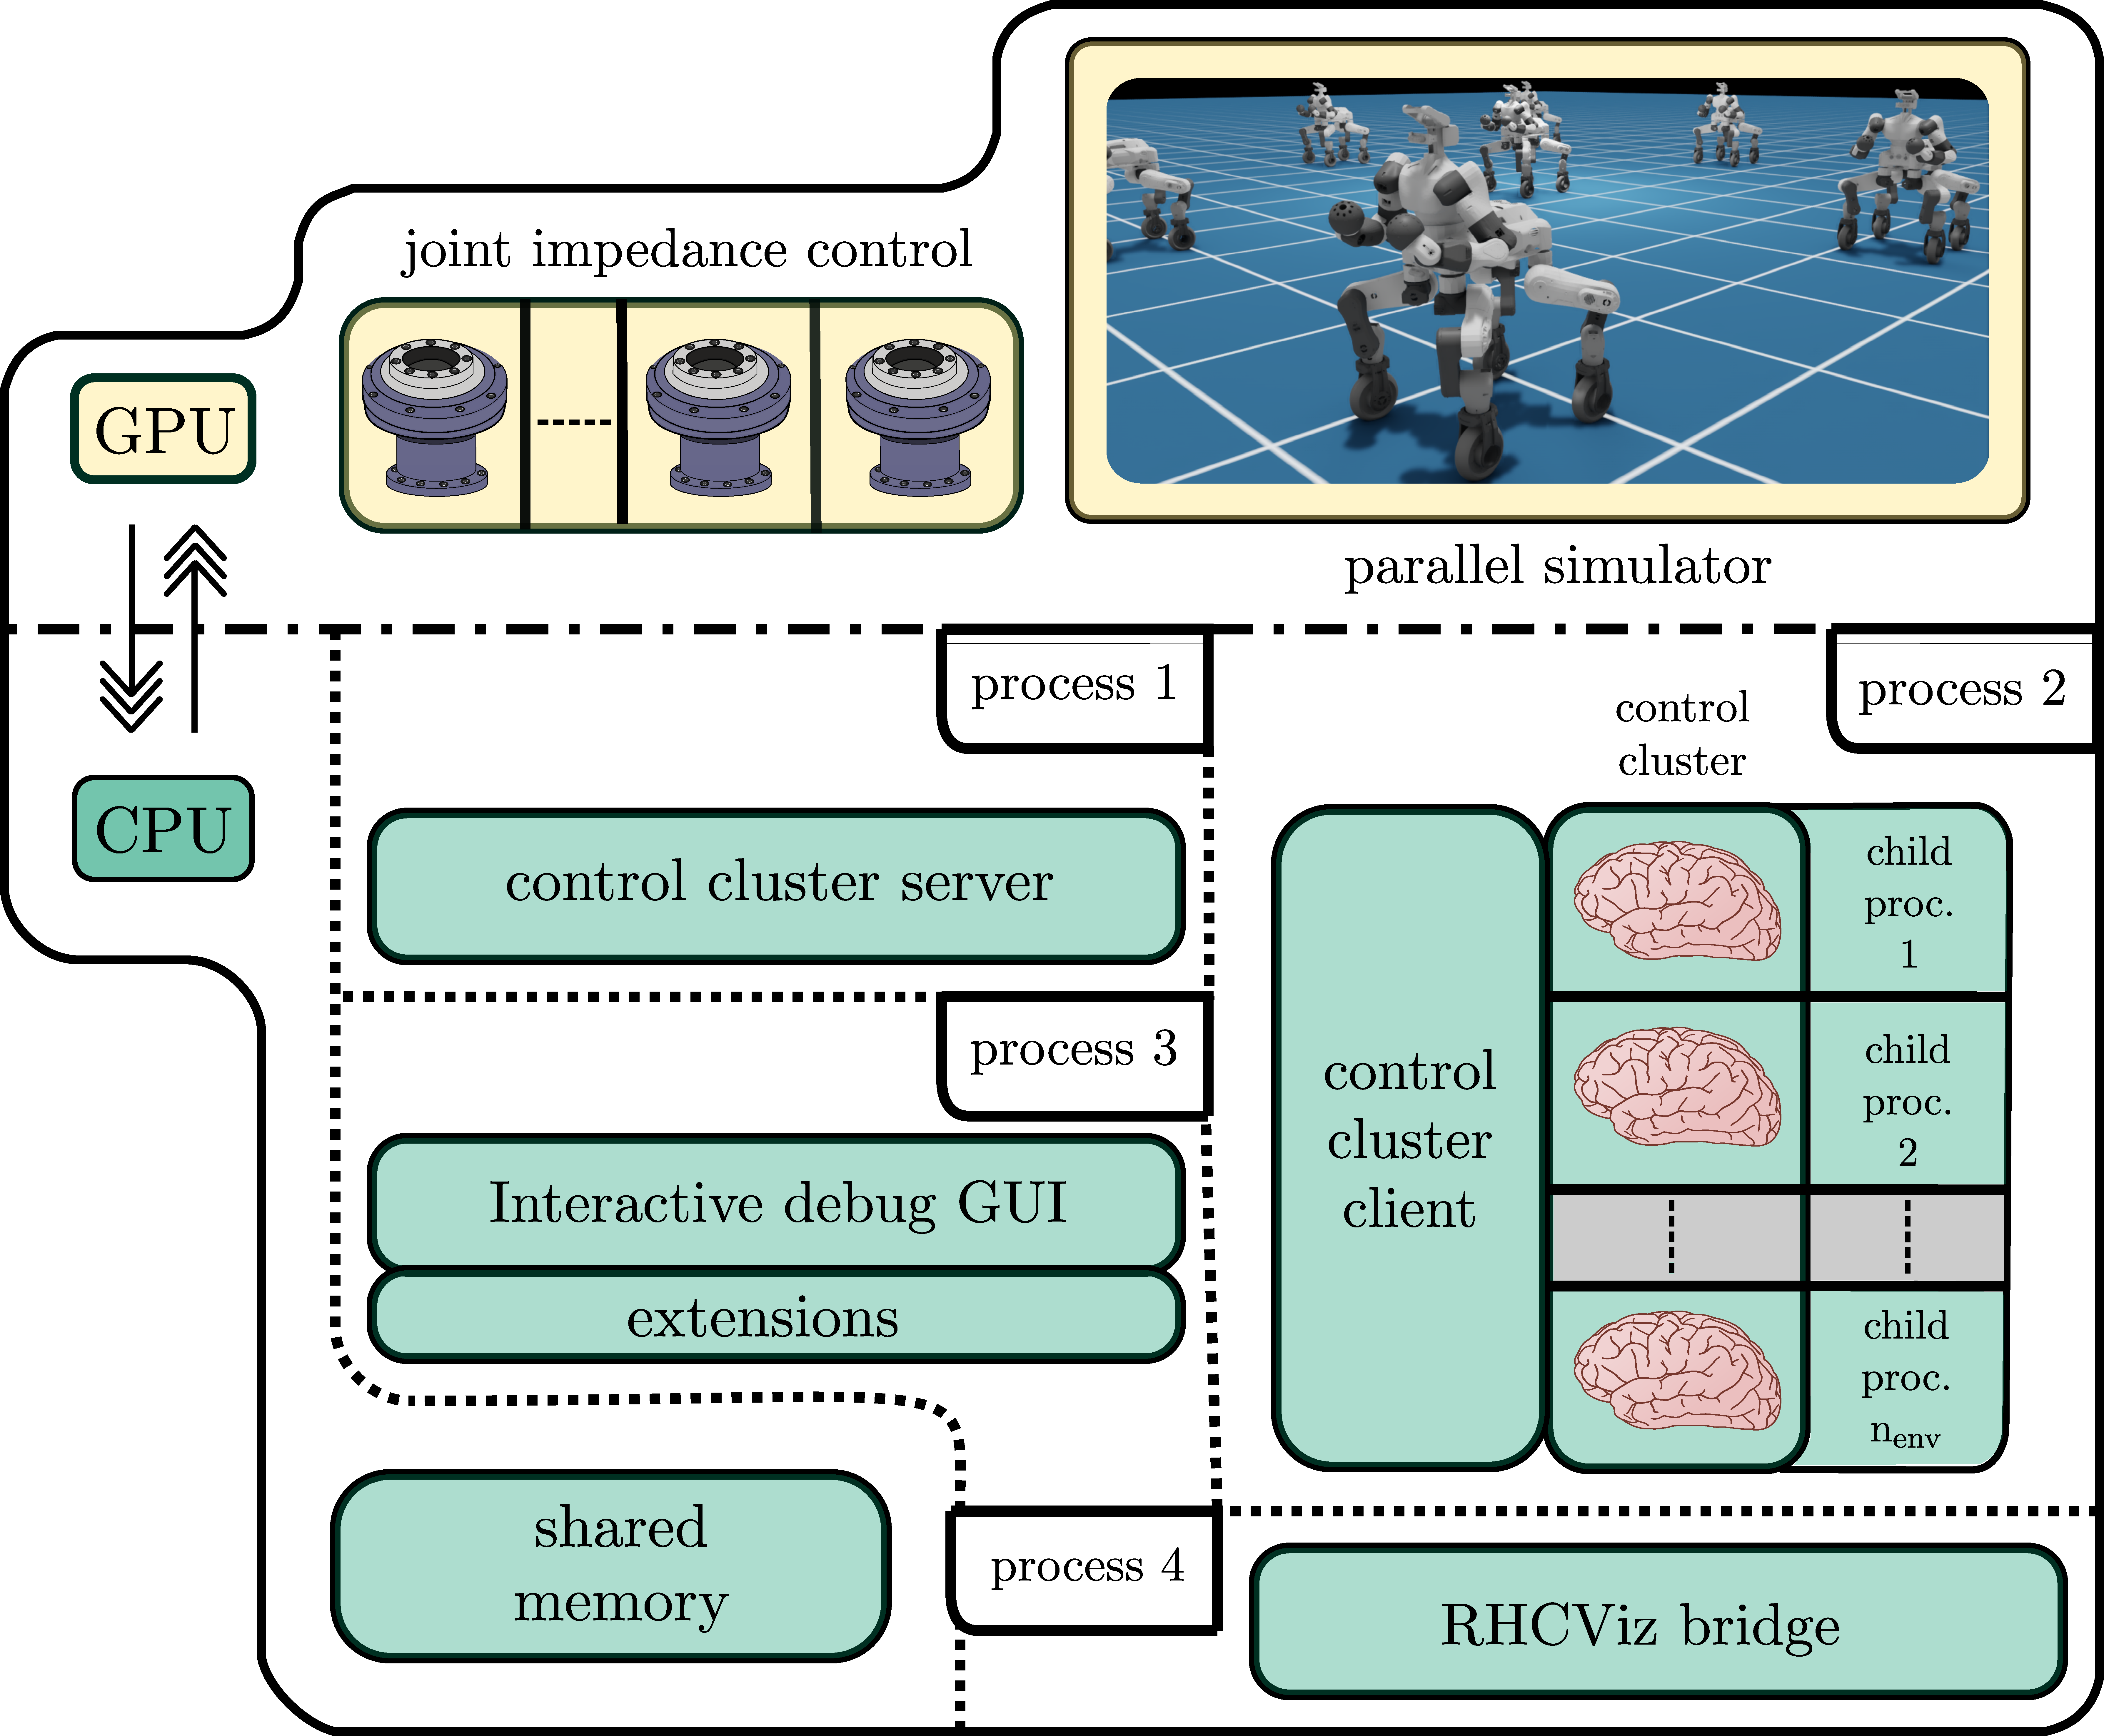
\includegraphics[width=1.0\columnwidth]{imgs/cocluster_arch.pdf}
	\caption{High-level overview of the software implementation of the training environment to which the agent is exposed: the robot in the simulator is controlled through a joint-level impedance controller, which is in turn used by a higher-level receding horizon controller. The agent can indirectly control the robot through the latter.}
	\label{fig:coclbridge_arch}
\end{figure}

\cite{rl:makoviychuk2021isaac}
\cite{rl:mujocoaccelereted2023}
\cite{frameworks:mittal2023orbit}
\cite{frameworks::horizon_to}

\cite{mystuff::lrhccontrol}
\cite{mystuff::omnirobogym}
\cite{mystuff::coclusterbridge}
\cite{mystuff::rhcviz}
\cite{mystuff::sharsoripcpp}